\section{Experiment}
%===================

Based on the working formula for $\K$, a Gaussian Na\"ive Bayes classifier was created and tested against 
an EMNIST \Hyperlink{https://drive.google.com/file/d/18ZY7I1ym0E9s2ecqjfvmPSGwlXzsNi2n}{dataset}
of over 370,000 grayscale 28x28 images of A--Z handwritten alphabets.
\begin{itemize}[noitemsep]
	\item Hence, our dataset had 26 classes (A--Z) with 784 features (pixels) each taking one of 256 values.
	\item The entire dataset was randomly divided into testing sets and training sets in 1:9 ratio.
	\item The classifier uses Gaussian distribution model despite the pixels taking discrete values -- because the training set may not have enough samples to plot the distribution of each pixel accurately.
	\item Smoothing factor $\xi \approx 2048$ was found to give the best results. This corresponds to the assumption of a minimum variance of $32^2$ in the values of the features of every class.
\end{itemize}
The results of one such experiment are presented in this section:\\
Python \& C++ codes for the classifier are available at \Hyperlink{https://github.com/s-rohit/naive-bayes}{Github}.

\subsection{Mean and Variance}
%-----------------------------
The mean and variance of the pixels each alphabet are presented as 28x28 grayscale images. \\
As expected, the mean represents ``what that alphabet on average looks like'', and the variance increases towards the edges and the protruding parts of each alphabet.
\begin{figure}[h]
	\centering
	\caption{Mean of pixel values of each alphabet (scaled).}\par
	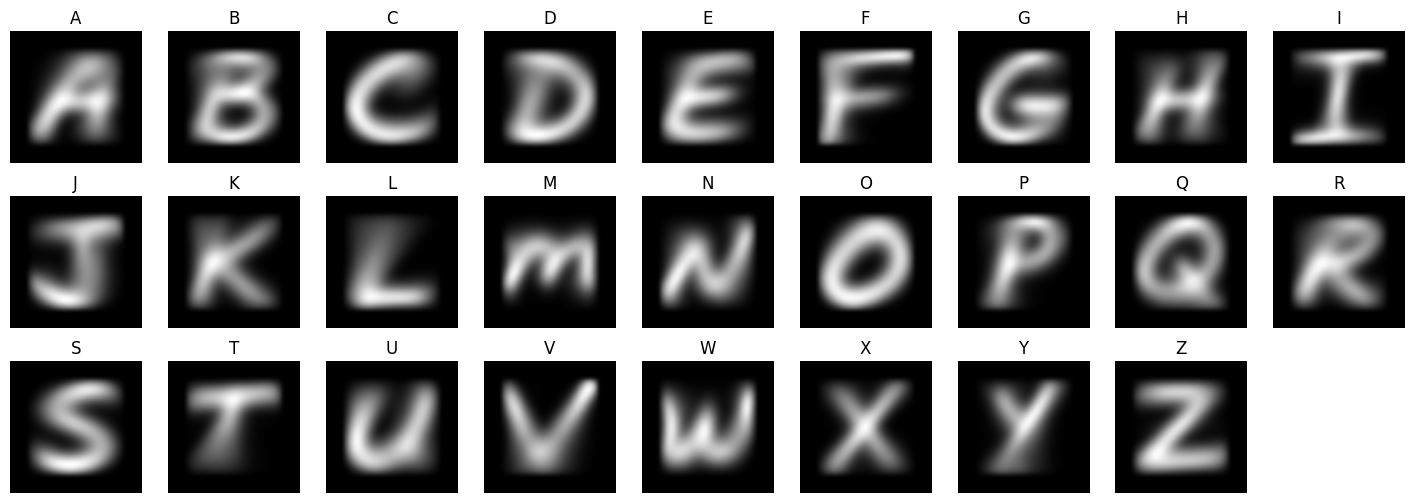
\includegraphics[width=0.725\textwidth]{fig/mean}
	\caption{Variance of pixel values of each alphabet (scaled).}\par
	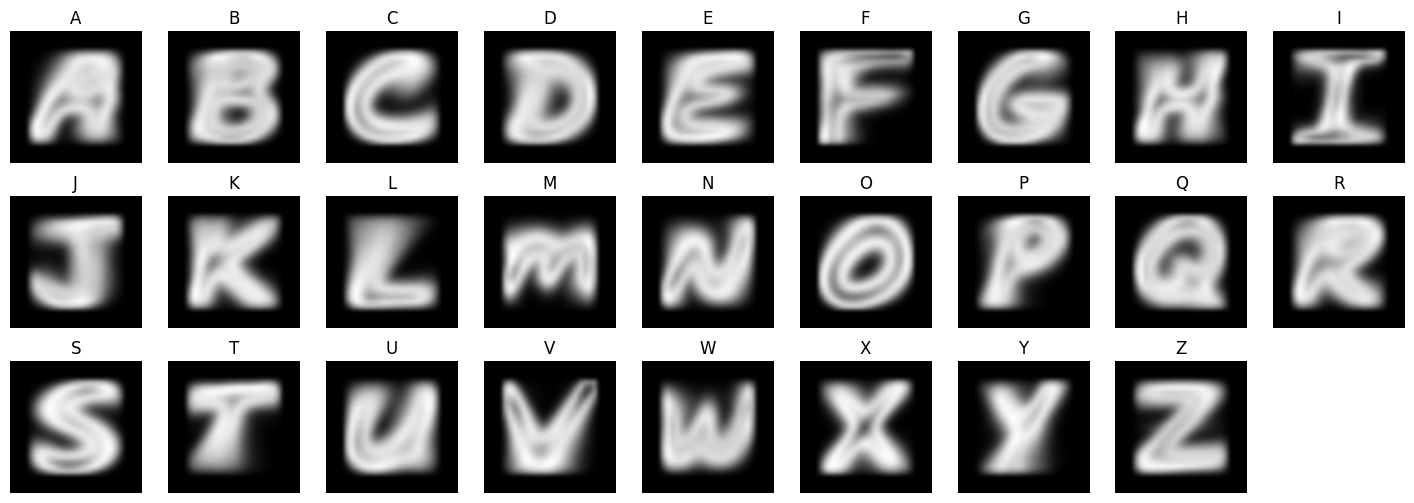
\includegraphics[width=0.725\textwidth]{fig/variance}
\end{figure}

\newpage
\subsection{Confusion matrix and Accuracy}
%----------------------------------------
As described in section 1, the overall and class-wise accuracy are found using the confusion matrix.
\begin{itemize}[nosep]
	\item Overall accuracy = trace of matrix $\div$ total sum
	\item Class-wise accuracy = value$_{ii}$ $\div$ row-wise sum
\end{itemize}
\begin{figure}[h]
	\centering
	\small
	\caption{Accuracy of prediction}\par
	\textbf{Overall accuracy $\approx 70.05\%$}\par\medskip
	\begin{tabu}{|c|c|c |c|c|c |c|c|c |}
		\tabucline-\rowfont\bfseries
		A        &  B      &  C      &  D      &  E      &  F      &  G      &  H      &  I     \\
		74.46\% & 71.78\% & 71.61\% & 69.44\% & 58.81\% & 87.59\% & 78.63\% & 44.46\% & 92.62\% \\ 
		\tabucline-\rowfont\bfseries
		J       &  K      &  L      &  M      &  N      &  O      &  P      &  Q      &  R      \\
		54.55\% & 60.84\% & 73.44\% & 88.69\% & 58.28\% & 82.72\% & 81.42\% & 75.93\% & 45.03\% \\ 
		\tabucline-\rowfont\bfseries
		S       &  T      &  U      &  V      &  W      &  X      &  Y      &  Z      & \\
		66.80\% & 72.14\% & 54.45\% & 88.98\% & 78.62\% & 61.39\% & 78.31\% & 56.03\% & \\
		\tabucline-
	\end{tabu}
	\par\bigskip
	\caption{Confusion matrix}\par
	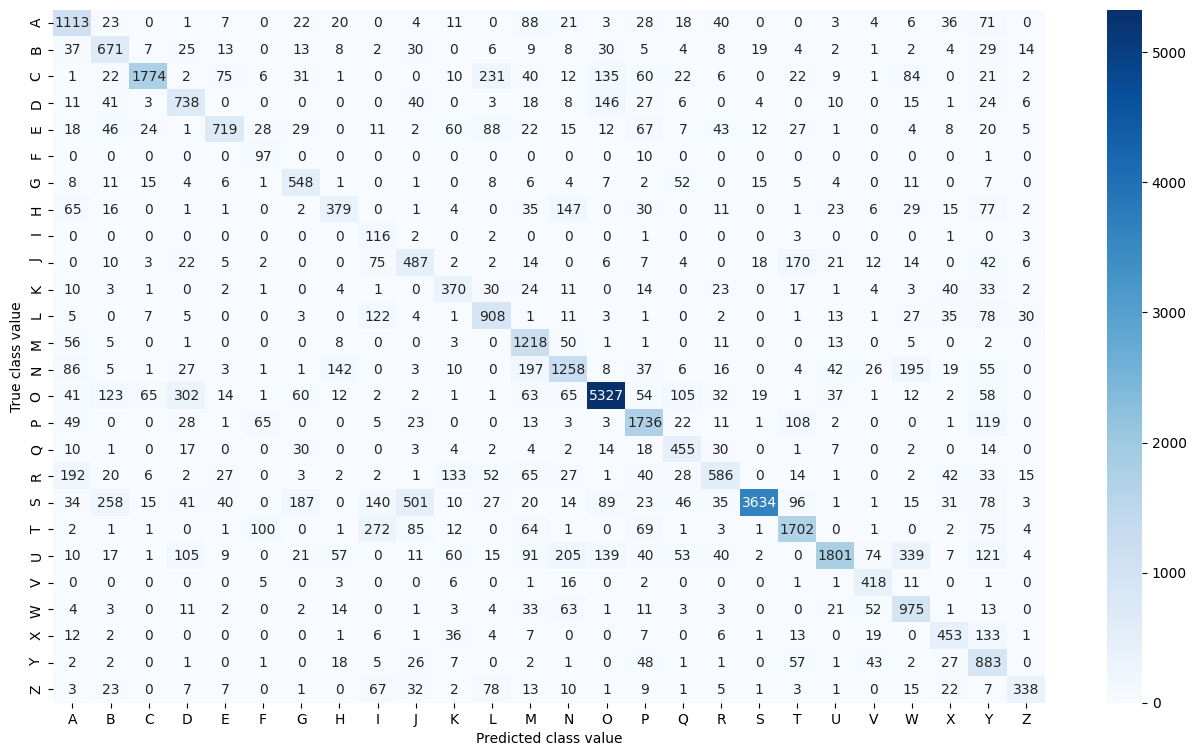
\includegraphics[width=0.99\textwidth, trim={0 0 5cm 0}]{fig/confusion}
\end{figure}

\textbf{Observations}
\begin{itemize}[itemsep=0pt]
	\item Letter `H' has the least accuracy, and is confused for `N' about a third of the time.
	\item Letter `R' has a low accuracy, and is often confused for `A' and `K'.
	\item Letters `F' and `I' seem to have high accuracy, but were not tested as much as others.
	\item Letters `O' and `S' were tested the most; letter `I' has the highest accuracy.
\end{itemize}